\documentclass[12pt]{article}
\usepackage[utf8]{inputenc}
\usepackage{csquotes}
\usepackage[ngerman]{babel}
\usepackage[backend=biber, style=apa, sorting=nty]{biblatex}
\renewcommand*{\bibfont}{\small}
\addbibresource{citation.bib}
\usepackage[T1]{fontenc}
\usepackage[top=2cm,left=3cm,right=2cm,bottom=2cm]{geometry}
\usepackage[parfill]{parskip}
\usepackage[font=normalsize]{caption}
\usepackage{hyperref}
\usepackage{multirow}
\usepackage{amsmath}
\usepackage{amssymb}
%% From HAW-Template
\usepackage{setspace}
\usepackage{listings}
\usepackage{graphicx} %% Important for including pictures
\graphicspath{{./images/}}
%% define colors in article
\usepackage{xcolor}
\definecolor{arsenic}{rgb}{0.23, 0.27, 0.29}
\definecolor{smokyblack}{rgb}{0.06, 0.05, 0.03}
\definecolor{coolblack}{rgb}{0.0, 0.18, 0.39}
\definecolor{mistyrose}{rgb}{1.0, 0.89, 0.88}
\hypersetup{
  colorlinks=true,
  linkcolor=black,
  filecolor=cyan,
  urlcolor=coolblack,
  citecolor=black,
}

%% \linespread{1.25} %% Paragraphs 1.5 lineheight
\onehalfspacing

%% \setmainfont{Arial}
\usepackage{uarial}
\renewcommand{\familydefault}{\sfdefault}

%% to set size of headings as normalsize 12pt
\usepackage{sectsty}
\sectionfont{\normalsize}
\subsectionfont{\normalsize}

%% to change space of headings to 0
\usepackage{titlesec}
\titlespacing*{\section}
{0pt}{12pt}{6pt}
\titlespacing*{\subsection}
{0pt}{6pt}{6pt}
\titlespacing*{\subsubsection}
{0pt}{6pt}{6pt}

%% set headers 
\usepackage{fancyhdr}
\pagestyle{fancy}
\fancyhf{}
\rhead{\textit{\footnotesize{Duy Nguyen. 2359864}}}
\rfoot{\thepage}
%% change paragraph margins
\usepackage{changepage}
\title{Vorstellung der Temperatursensoren und deren Eignung für Feinstaubmessprojekt}
\author{Duy Nguyen}

%% Begin document
\begin{document}
\pagestyle{empty}
\color{smokyblack}

\setlength{\parskip}{1ex}
\begin{table}[t]
  \begin{center}
    \begin{tabular}{p{0.7\textwidth}r}
      \small{HAW-Hamburg} & \multirow{4}{*}{
\includegraphics[width=4.6cm]{haw-logo}} \\
      \small{Vorlesung Messtechnik} &  \\
      \small{Sommersemester 2021} & \\
      \small{Prof. Dr. Carsten Frank} & 
    \end{tabular} 
  \end{center}
\end{table}

\vspace{2cm}

\textsf{\textit{\Large{Hausarbeit}}}

\color{arsenic}
\textsf{\textbf{\huge{Vorstellung der Temperatursensoren und deren Eignung für Feinstaubmessprojekt}}}
\setlength{\parskip}{0.8em}
\color{smokyblack}
%% Add abstract paragraph
\vspace{-2em}

\begin{adjustwidth}{3em}{0pt}
\begin{flushleft}
	\textit{Duy Nguyen} 

  \vspace{-12pt}

  \textit{\footnotesize{Feinstaubsgruppe: Duy Nguyen, Ferris Fensky, Dennis Dick}}
\end{flushleft}
\end{adjustwidth}

\tableofcontents
\newpage
\listoffigures
\addcontentsline{toc}{section}{Abbildungsverzeichnis}
\listoftables
\addcontentsline{toc}{section}{Tabellenverzeichnis}

%% Uncomment these lines to input manually list of abbreviations as IV from external file
%% \input{abbreviationpage}
%% \addcontentsline{toc}{section}{List of abbreviations}

\newpage
\pagestyle{fancy}
\section{Temperatursensoren}
\label{sec:temperatursensoren}

Wir wollen in unserem Projekt Feinstaubmessung die Temperatur messen. Die Temperatur an Feinstaubmessgerät (mehr genauer ist auf Lichtsensor (Fotodiode) des Geräts) ist interessant. Die gewählter Temperatursbereich ist von -20°C bis zum 40°C. Es wurde informiert, dass Mindesttemperatur in Deutsch -20 Grad und Maximaltemperatur ungefähr 45 Grad, in den Schatten ist aber ein bisschen weniger in Sommer und der Wert 40 Grad wurde gewählt, um den Bereich einzugrenzen. Die Messgenauigkeit ist 0,1°C.

\subsection{PT100}
\subsubsection{Einleitung und Funktionsprinzip}

In allen Leitern entsteht durch Erhitzung ein Effekt, was den Widerstand des Leiters erhöht. Das Effekt wurde dann genutzt, um das PT100-Sensor herzustellen und Temperatur in Abhängigkeit von dem Widerstand des Leiters (Metalldraht/Metallstücke) zu messen. Die Elektronen wurden von Metallatomen freigesetzt durch angeregten Zustand und bauen das Leitungsband zusammen, in dem die sich miteinander stoßen und bewegen. Dadurch ist Strom erschaffen. Durch Erwärmung steigt die Temperatur, gleichzeitig werden die Elektronen aus der Bahn geworfen und im Leitungsband befinden sich weniger Elektronen, der Widerstand steigt. Das Effekt wurde auch so genannt, dass es Gitterschwingung in Moleküle des Kristallgitters von Metall ist.(\cite{Frank.}, \cite{W.GopelJ.HesseJ.N.Zemel.1989}, \cite{L.v.Kortvelyessy.1987})

\subsubsection{Beispiel PT100 Sensor}

\begin{figure}[h]
  \centering
  \label{fig:pt100m213}
  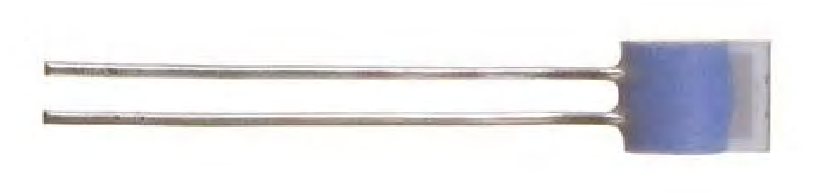
\includegraphics[width=0.5\textwidth]{PT100M213}
  \caption{PT100 Serie M213 (\cite{MouserElectronics.2021c})}
\end{figure}

\begin{figure}[h]
  \centering
  \label{fig:pt100schaltung}
  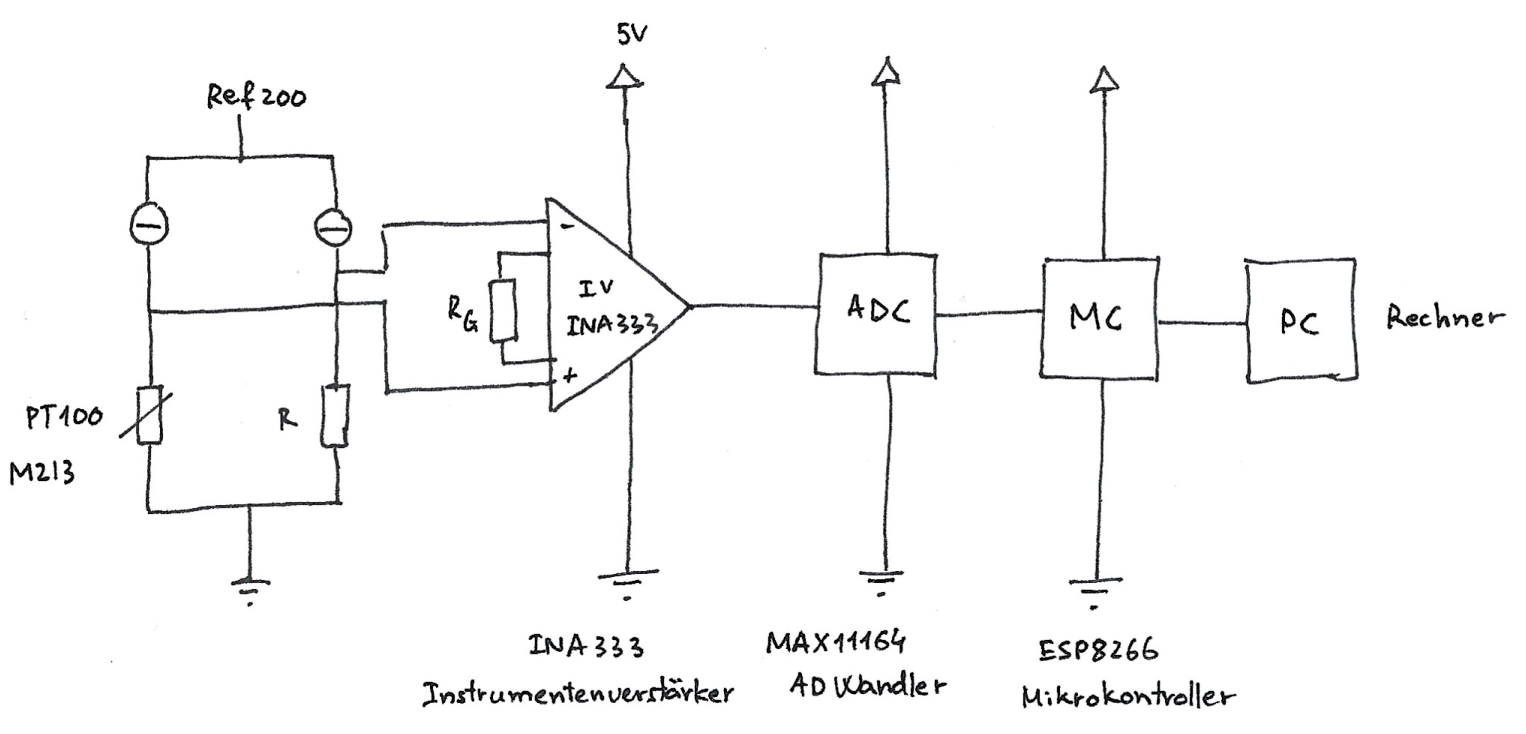
\includegraphics[width=0.9\textwidth]{PT100Schaltung}
  \caption{Schaltung PT100 in Betrieb }
\end{figure}

Hier haben wir der Sensor PT100 M213 genommen. Der Preis beträgt 5,46€ für ein Stück. (\cite{MouserElectronics.2021c}) Datasheet: (\cite{Pustelnik.2019}). Temperaturmessbereich befindet sich von -70°C bis 500°C. Bei 0°C ist der Widerstand 100$\Omega$.

Der PT100 hat die Widerstandsänderung proportional zu der Temperatur und daher sehr gut geeignet für Empfänger bzw. Studie über RTD (resistance temperature detectors) allgemein. Der hat auch langen Lebensdauer und ist verfügbar kalibriert mit verschiedenen Genauigkeiten. 

Hier haben wir eine REF200 Duale Stromquelle genutzt, um zwei jeweils 100$\mu A$ herzustellen. Die Versorgung sind für den PT100 Temperatursensor und einen Offsetwiderstand eingestellt.

Die Formel (\ref{Rpt100}) wird dann für die Berechnung des Widerstand des PT100 verwendet:

\begin{equation}\label{Rpt100}
R_\upsilon = R_0 * (1 + 3,85.10^{-3} * \frac{1}{K} * T) 
\end{equation}

Dann haben wir: 

\begin{center}
$R_{\upsilon bei -20°C} = 100\Omega * (1 + 3,85.10^{-3} * \frac{1}{K} * -20) = 92,3\Omega$

$R_{\upsilon bei 40°C} = 100\Omega * (1 + 3,85.10^{-3} * \frac{1}{K} * 40) = 115,4\Omega$
\end{center}

Der Offsetwiderstand 

\begin{center}
  $R_1 = R_{PT100 bei -20°C} = 92,3\Omega$
\end{center}

Bei -20°C haben wir beim Eingang des Verstärkers: 

\begin{center}
  $V_{in-20} = 92,3\Omega * 100 * 10^{-6}A = 9,23mV$ 
\end{center}

Bei +40°C haben wir beim Eingang des Verstärkers: 

\begin{center}
  $V_{in40} = 115,4\Omega * 100 * 10^{-6}A = 11,54mV$ 
\end{center}

Die Differenz wäre:

\begin{center}
 $V_{in40} - V_{in-20} = 2,31mV$
\end{center}

Der AD Wandler MAX11164 wurde genutzt, um dieses Spannungssignal in Digitalsignal zu wandlern. Der hat eine Referenzspannung von 4,096V und daher brauchen wir die Spannungsdifferenz beim Eingang des Verstärkers maximal in Faktor von $\frac{4,096}{2,31*10^{-3}} = 1773$ zu verstärken. 

Der Instrumentenverstärker INA333 wurde verwendet, um das Signal in Faktor von 1000-mal zu verstärken. Dafür brauchen wir $R_G = 100,1\Omega$ (siehe Schaltung). (\cite{TexasInstruments.2020})

Die Differenz beim Ausgang des Verstärkers ist gleich beim Eingang des AD Wandler, nämlich den Wert von 0 bis 2,31V beträgt es. Für unserem Messbereich wäre: $\frac{2,31}{40 - -20} = 0,0385V = 38,5 \frac{mV}{^{\circ} C}$

MAX11164 hat $\frac{4,096}{2^{16}} = 0,0625 \frac{mV}{bit}$ (\cite{MaximIntegratedProducts.2015})

Das führt zu einer Auflösung von $\frac{0,0625mV/bit}{38,5mV/^{\circ} C} = 0,0016 ^{\circ} C/bit < 0,1 ^{\circ} C/bit$ (gewünschte Auflösung). Das erfüllt die Erwartung und ist zu sehen, dass in reale Praxis die Bauteile miteinander harmonieren können.
\subsection{NTC Thermistor}

\subsubsection{Einleitung und Funktionsprinzip}

Negative Temperatur Koeffizient Thermistoren sind Widerstände mit einem negativen Temperaturkoeffizienten. Das heißt, dass der Widerstand mit einer steigenden Temperatur sinkt. NTC-Thermistoren lassen sich aus Halbleiter herstellen und konfigurieren, dass die hohe Widerstandschwankung im Vergleich mit kleiner Änderung in der Temperatur haben. 

Durch Verwendung eines Gleichstroms, der durch Thermistor geleitet wird, ist der erzeugte Spannungsabfall zu messen.

Halbleiter haben bei Absolut-Null-Grad keine Elektronen auf Leitungsband und bleiben inaktiv. Wenn die Temperatur sich erhöht, kovalente Bindungen in Halbleiter wird unstabil und gebrochen, setzen die Elektronen frei, jedes freie Elektron formt eine Lücke in Valenzband und die haben genug Energie, um über die Bandlücke zu Leitungsband zu springen. Je hohe Temperatur, desto mehr Elektronen springen in Leitungsband und formen Löcher in Valenzband, gibts dann Platz für andere Elektronen in Valenzband zu bewegen und Strom lässt sich durch Halbleiter fließen. (\cite{TEConnectivity.2021}, \cite{Frank.})

\subsubsection{Beispiel NTC Thermistor}

\begin{figure}[h]
  \centering
  \label{fig:NTC}
  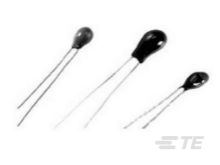
\includegraphics[width=0.2\textwidth]{NTC44008RC}
  \caption{NTC Thermistor Modell 44008RC mit Epoxydbeschichtung (\cite{TEConnectivity.2021c})}
\end{figure}

\begin{figure}[h]
  \centering
  \label{fig:ntcschaltung}
  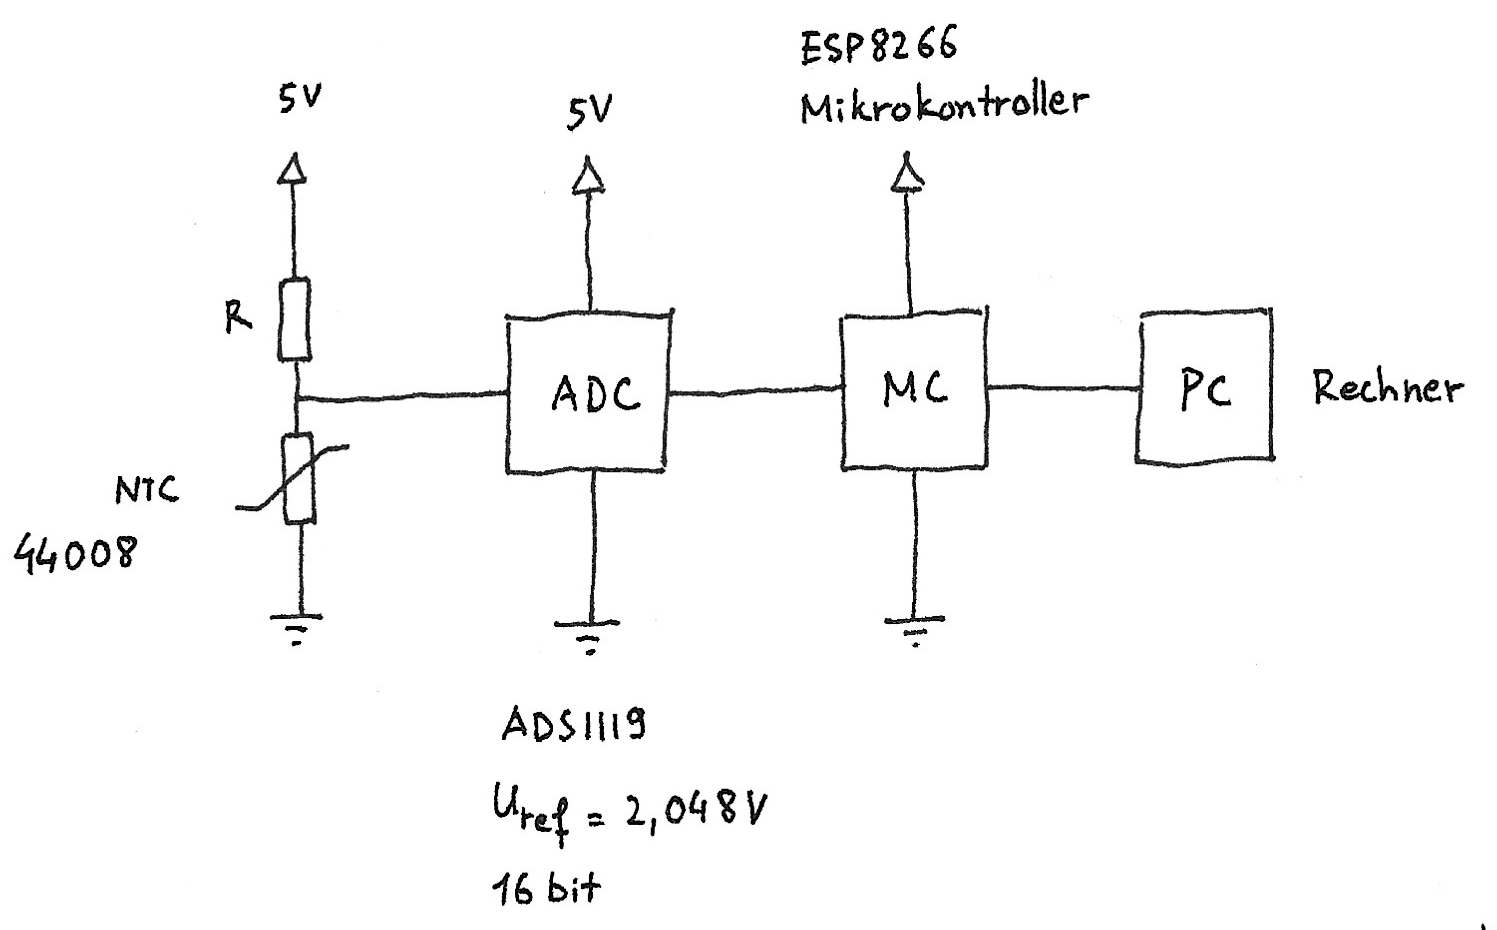
\includegraphics[width=0.9\textwidth]{NTCSchaltung}
  \caption{Schaltung NTC Thermistor in Betrieb }
\end{figure}

Der NTC Thermistor Model 44008 wurde gewählt. Sein Widerstand bei 25°C beträgt $R_{25} = 30000\Omega$. Der Preis beträgt 7,54€ pro Stück (\cite{TEConnectivity.2021c}). Datenblatt unter (\cite{TEConnectivity.2016}).

Da die Kennlinie des NTC nicht linear ist, hier teilen wir den Messbereich in zwei Bereiche, nämlich oberer Teil (von 39 bis 40°C) und unterer Teil (von -19 bis -20°C). Für beste Leistung, der Wert von $R$ (siehe Schaltung) ist so gewählt, dass das Verhältnis zwischen $R$ und $R_{Thermistor_{Max}}$ gleich mit dem Verhältnis zwischen $R$ und $R_{Thermistor_{Min}}$. Die Gleichung (\ref{Rref}) ist dafür geeignet: (\cite{TexasInstruments.2018})

\begin{equation}
  R^2 = R_{Thermistor_{Min}} * R_{Thermistor_{Max}}
\end{equation}
entspricht
\begin{equation}\label{Rref}
  R = \sqrt{R_{Thermistor_{Min}} * R_{Thermistor_{Max}}}
\end{equation}


\begin{table}[h]
  \caption{\normalsize{NTC Widerstände in Abhängigkeit von Temperatur (\cite{TEConnectivity.2016})}}
  \begin{center}
    \begin{tabular}{r|r}
    T [°C] & R [$k\Omega$] \\
    \hline
    -20 & 271,2 \\
    -19 & 265,5 \\
    40 & 16,15 \\
    39 & 16,80 \\
    \end{tabular} 
  \end{center}
\end{table}

Für oberen Bereich von 39°C bis 40°C: 
\begin{center}
$R = \sqrt{271,2k\Omega * 256,5k\Omega}$, also entspricht $R = 263,75k\Omega$
\end{center}

Für unteren Bereich von -19°C bis -20°C: 
\begin{center}
$R = \sqrt{16,15k\Omega * 16,80k\Omega}$, also entspricht $R = 16,47k\Omega$
\end{center}

Mit Formel (\ref{Rref}) ist R von $R_{NTC bei -20°C} = 271,2k\Omega$ und $R_{NTC bei 40°C} = 16,15k\Omega$ zu berechnen, der Wert beträgt $R = 66,2k\Omega$.

Die Formel (\ref{Vin}) (\cite{TexasInstruments.2018}) drückt aus, wie die Inputspannung des AD Wandler und Referenzspannung sich mit den Widerständen beziehen: 

\begin{equation}\label{Vin}
  V_{in} = \frac{R_{Thermistor}}{R_{Thermistor} + R} * V_{REF}
\end{equation}

Dadurch folgen die Berechnungen:
\begin{center}
$V_{ADC input bei -20^\circ C} = \frac{R_{NTC}}{R_{NTC} + R} * V_{REF} = \frac{271,2k\Omega}{271,2k\Omega + 263,75k\Omega} * 2,048V = 1,038V$ 

$V_{ADC input bei -19^\circ C} = \frac{R_{NTC}}{R_{NTC} + R} * V_{REF} = \frac{256,5k\Omega}{256,5k\Omega + 263,75k\Omega} * 2,048V = 1,0097V$

$\Delta V = 0,02827 V/^\circ C = 28,27mV/^\circ C$ 

$V_{ADC input bei +40^\circ C} = \frac{R_{NTC}}{R_{NTC} + R} * V_{REF} = \frac{16,15k\Omega}{16,15k\Omega + 16,47k\Omega} * 2,048V = 1,014V$ 

$V_{ADC input bei -39^\circ C} = \frac{R_{NTC}}{R_{NTC} + R} * V_{REF} = \frac{16,80k\Omega}{16,80k\Omega + 16,47k\Omega} * 2,048V = 1,034V$ 

$\Delta V = 0,02016 V/^\circ C = 20,16mV/^\circ C$ 

\end{center}

AD Wandler ADS1119 hat $\frac{2,048V}{2^{16}} = 0,03125 \frac{mV}{bit}$ (\cite{TexasInstruments.2018})

Das führt zu eine Auflösung von $\frac{0,03125/bit}{28,27mV/^{\circ} C} = 0,0011 ^{\circ} C/bit < 0,1 ^{\circ} C/bit$ (gewünschte Auflösung) in oberem Bereich und $0,00155 ^{\circ} C/bit < 0,1 ^{\circ} C$ im unterem Bereich. Dadurch lässt sich ausgesagt werden, dass die Auflösungen nicht viel von einander abweichern und in Ordnung sind.  Es wurde nochmal durch Formel (\ref{Vin}) überprüft werden und die Auflösung von $0,0015625^\circ C/bit$ wurde ausgerechnet. Das erfüllt die Erwartung und ist zu sehen, dass in realen Praxis die Bauteile mit einander harmonieren können.

\subsection{Thermoelement Typ K}

\subsubsection{Einleitung und Funktionsprinzip}

Thermoelemente beruhen auf dem thermoelektrischen Effekt. Sie liefern eine weitgehend  temperaturproportionale elektrische Spannung. Ein Thermoelement besteht meist aus zwei Metalldrähte aus unterschiedlichem Metall z.B aus Nickel und Nickelchrom, Platin und Platinrhodium, ... Am Ende beides Drahten werden zusammengeschweißt. Da wird es erwärmt.

Wenn die Temperatur steigt, schwingen die Metallionen immer stärker und nehmen thermische Energie auf. Die Metallatomen können aber nicht ihren Platz verlassen (T < Schmelzpunkt), die Elektronen an erwärmter Stelle werden mit hoher Geschwindigkeit bewegen und geschoben, dass die in den kalten Teil des Drahtes fließen. Der thermoelektrische Effekt besteht darin, dass der erwärmte Teil eines Drahtes elektronenärmer wird, der kältere Teil dieses Drahtes aber elektronenreicher. Dadurch wird der wärmere Teil positiv und der kältere Teil negativ aufgeladen. (\cite{L.v.Kortvelyessy.1987}). Je höher die Temperatur steigt, desto mehr Elektronen bewegen sich auf die kalte Seite des Leiters. So wird sich zwischen den nicht gebundenen Enden der Leiters eine Spannungsdifferenz einstellen. (Seebeck-Effekt)

Die Thermospannung an kaltem Ende des Drahtens können dann durch Messung bestimmt werden und damit eine geschlossene Schaltung erzeugen. (siehe Abbildung thermoelektrische Effekt von \cite{L.v.Kortvelyessy.1987})

\begin{figure}[h]
  \centering
  \label{fig:thermoelektrischerEffekt}
  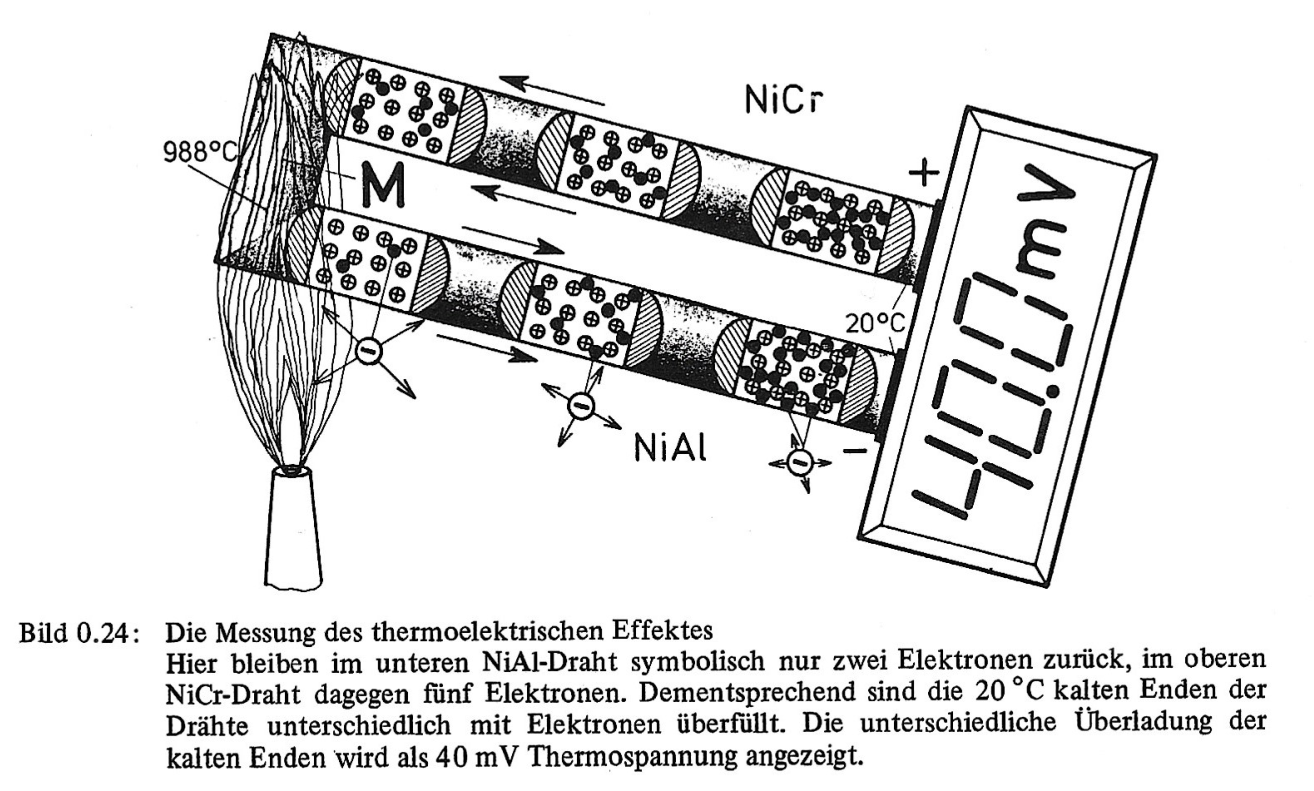
\includegraphics[width=0.8\textwidth]{thermoelektrischerEffekt}
  \caption{Die Messung des elektrischen Effektes (\cite{L.v.Kortvelyessy.1987})}
\end{figure}

\subsubsection{Beispiel Thermoelement Typ K}

\begin{figure}[h]
  \centering
  \label{fig:thermoelementtypK}
  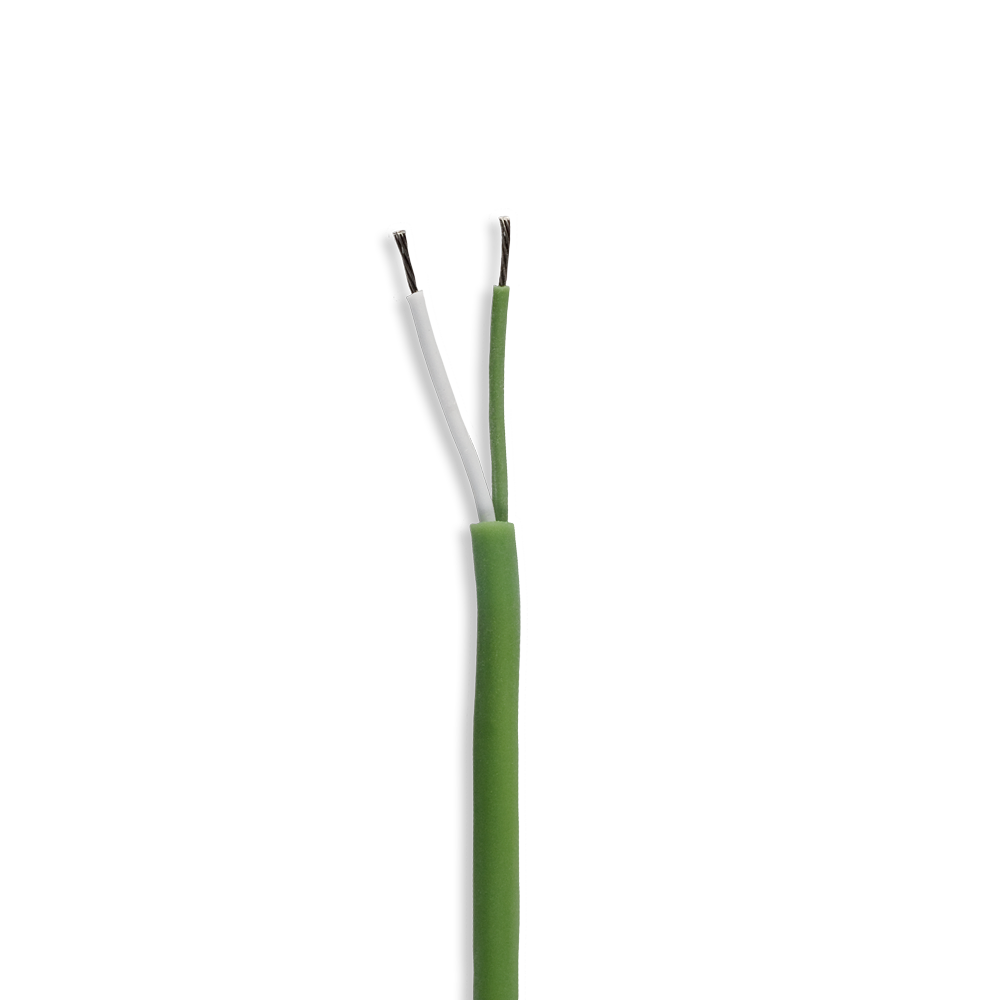
\includegraphics[width=0.3\textwidth]{thermoelement_typ_k_pvc}
  \caption{Thermoelement Typ K aus NiCr-Ni, Leiterisolation PVC (\cite{Therma.2020})}
\end{figure}

\begin{figure}[h]
  \centering
  \label{fig:ThermoelementSchaltung}
  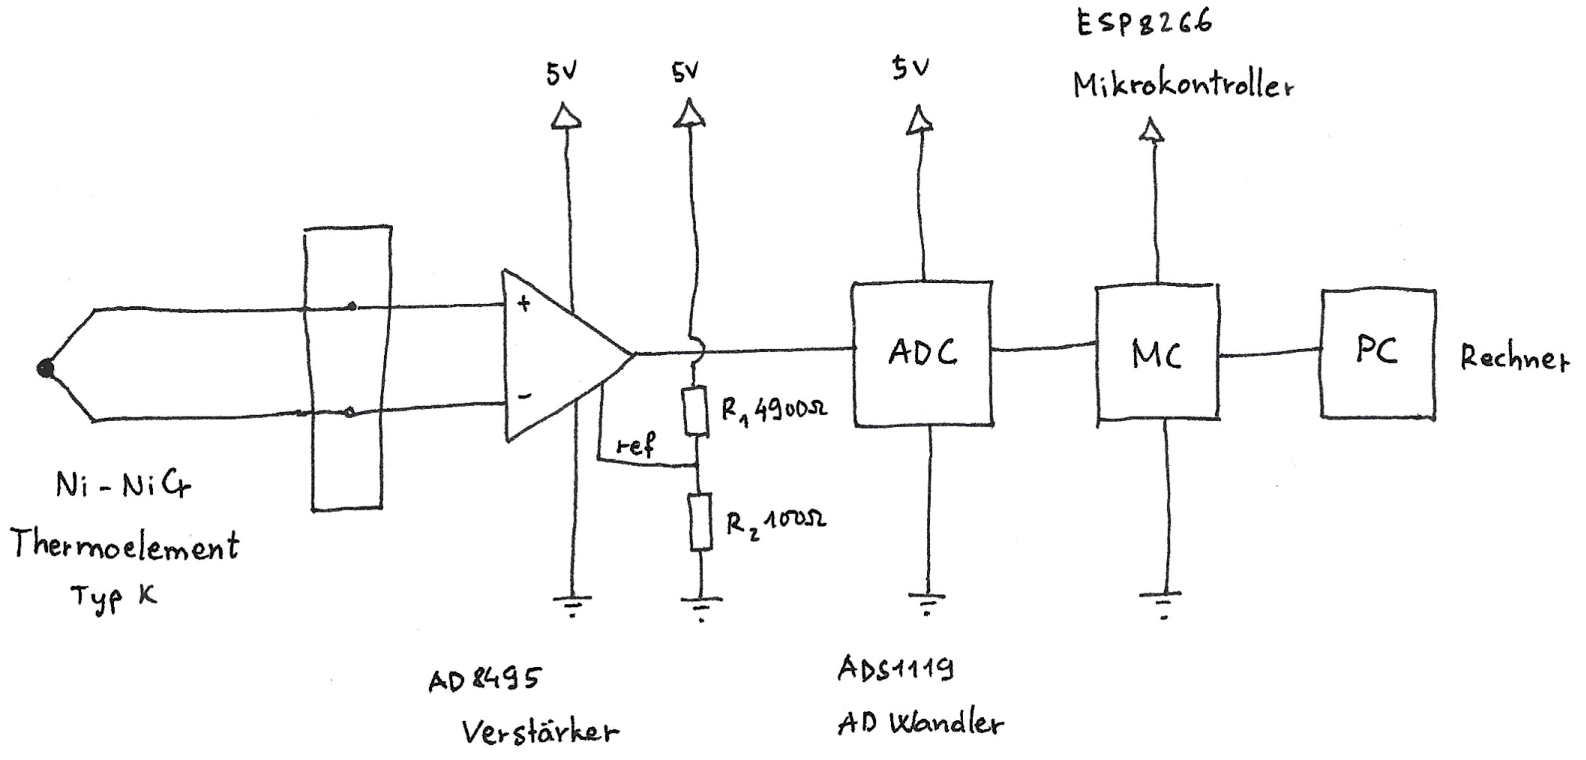
\includegraphics[width=0.9\textwidth]{ThermoelementSchaltung}
  \caption{Schaltung Thermoelement Typ K in Betrieb}
\end{figure}

Das Thermoelement Typ K ist gewählt. Es besteht aus zwei Metalldrahte aus Nickel und Nickelchrom. Der Preis beträgt 10,50€ pro Stück mit PVC-Mantel (\cite{Therma.2020}). Datenblatt (\cite{Zacharias.2021}, \cite{NIST.2008}). 

\begin{table}[h]
  \caption{\normalsize{Thermospannung von Thermoelement Typ K in Abhängigkeit von Temperatur (\cite{NIST.2008})}}
  \label{thermospanung}
  \begin{center}
    \begin{tabular}{r|r}
    T [°C] & V [mV] \\
    \hline
    -20 & -0,778 \\
    -19 & -0,739 \\
    40 & 1,612 \\
    39 & 1,571 \\
    \end{tabular} 
  \end{center}
\end{table}

Es ist hier zu sehen, dass die Thermospannung sehr klein und negativ. (siehe Tabelle \ref{thermospanung}) Deswegen ist der AD8495 Verstärker genutzt, der ist schon für Thermoelement Typ K geeignet und integriert, damit wir große Ausgangsspannungen und eine lineare Kennlinie haben können. Das Thermoelement ist mit kalibrierter Temperaturvergleichsstelle zusammen verglichen, hier in Aufbau der AD8495 zu sehen (Cold Junction Compensation, \cite{AnalogDevicesInc..2018}). Bei 0°C liefert der Verstärker eine Ausgangsspannung von 0V und je 1°C steigt/sinkt die Spannung um 5mV. Das heißt folgendes, bei -20°C entsteht eine Spannung von -100mV und 40°C 200mV. Ein Offset von 100mV ist gebraucht, um die 0V Niveau zu -20°C Temperatursgrenzwert zu bringen. Der PIN REF des Verstärker AD8495 ist gebraucht. (siehe Schaltung $U_{Ref} = U_{R_2} = 100mV$). Davon gelten bei -20°C 0mV, 0°C 100mV und 40°C 300mV. 

Die Ausgangsspannung des Verstärkers ist Eingangsspannung des AD Wandlers. Hier wurde wieder der ADS1119 genutzt mit 0,03125mV/bit (\cite{TexasInstruments.2018}). Als die Spannung von 0 bis 0,3V schwingt und 5mV entspricht 1°C , haben wir die Auflösung von: 

\begin{center}
  $\frac{0,03125mV/bit}{5mV/^\circ C} = 0,00625 ^\circ C/bit < 0,1^\circ C$
\end{center}

Das erfüllt die Erwartung und ist zu sehen, dass in realen Praxis die Bauteile mit einander harmonieren können.

\section{Prüfung der Eignung von Temperatursensoren fürs Feinstaubmessprojekt}

Der PT100 wurde nach Diskussion gewählt. Das Feinstaubmessgerät wird dann in Schatten eingestellt, da lässt sich direkte Sonnenstrahlung vermeiden werden und hohe Erhitzung von Messgerät allgemein und die Fotodiode spezifisch würde vermindert. Mit hoher Lebensdauer wird der PT100 und auch seine Messschaltung überleben und konstant betreiben. Die Schaltung ist ein bisschen kompliziert, dass wir doch einen Instrumentenverstärker und Anpassung des Messbereichs brauchen, aber mit der linearen Kennlinie lässt sich die Werte leichter und anfängerfreundlicher berechnen bzw. programmieren. Die Temperatur ist hier in dem Fall ein Faktor, was mit der Luftfeuchtigkeit mitspielt und die Messung von Feinstaubpartikeln beeinflusst. Deswegen ist eine einfache, sichere und geprüfte Temperaturmessung sehr hilfreich, dass wir gut mit Luftfeuchtigkeitswerte bzw. Feinstaubswerte PM2.5 PM10,... vergleichen können.

\newpage
%% printbibliography
\printbibliography
\addcontentsline{toc}{section}{Literatur}
%% Umcomment these 4 lines to input \bibliography manually from other file
%% \newpage
%% \input{bibliography}
\begin{center}
\hyperref[sec:temperatursensoren]{\large{$\uparrow$}}
\end{center}
\newpage
\pagestyle{fancy}
\textbf{Eigenständigkeitserklärung}

\vspace{6pt}

Hiermit versichere ich, dass ich den vorliegenden Bericht selbstständig und nur mit den angegebenen Hilfsmitteln verfasst habe. Alle Passagen, die ich wörtlich aus der Literatur oder aus anderen Quellen wie z. B. Internetseiten übernommen habe, habe ich deutlich als Zitat mit Angabe der Quelle kenntlich gemacht. 

\begin{flushright}
	\today

	
	Duy Nguyen
\end{flushright}

\addcontentsline{toc}{section}{Eigenständigkeitserklärung}
\end{document}
